\documentclass[xetex,mathserif,serif]{beamer}
\usepackage{polyglossia}
\setdefaultlanguage[babelshorthands=true]{russian}
\usepackage{minted}

\useoutertheme{infolines}

\setmainfont{FreeSans}
\newfontfamily{\russianfonttt}{FreeSans}

\definecolor{links}{HTML}{2A1B81}
\hypersetup{colorlinks,linkcolor=,urlcolor=links}

\title{Курсовые работы на кафедре СП}
\subtitle{Регламент, требования, рекомендации}
\author[Юрий Литвинов]{Юрий Литвинов \newline \textcolor{gray}{\small\texttt{yurii.litvinov@gmail.com}}}
\date{12.09.2019г}

\begin{document}
	
	\frame{\titlepage}

	\begin{frame}
		\frametitle{Что такое курсовая}
		\begin{itemize}
			\item Научно-исследовательская работа
			\begin{itemize}
				\item Решение более-менее научной задачи
				\item Отчёт по курсовой работе
				\item Код (опционально, но желательно)
			\end{itemize}
			\item По формату близка к научной статье и выступлению на конференции
			\item Тема должна быть интересна кафедре (``программирование для программистов'')
		\end{itemize}
	\end{frame}

	\begin{frame}
		\frametitle{Сроки}
		\begin{itemize}
			\item Сентябрь-октябрь --- выбор темы
			\item Ноябрь --- утверждение темы на кафедре, табличка с темами и научниками
			\item Середина декабря --- промежуточный отчёт (введение, постановка задачи, обзор, текущие продвижения)
			\item Зачёт по курсовой работе (по отчёту)
			\item Начало мая --- предзащита
			\item Конец мая --- защита
		\end{itemize}
	\end{frame}

	\begin{frame}
		\frametitle{Требования}
		\begin{itemize}
			\item Отчёт (итоговый)
			\begin{itemize}
				\item Порядка 20 страниц
				\item Сдаётся за две недели до защиты
				\item Положительная рецензия на отчёт
			\end{itemize}
			\item Доклад
			\begin{itemize}
				\item Порядка 5-7 минут
			\end{itemize}
			\item Отзыв научного руководителя с рекомендуемой оценкой
			\item Код --- open source (желательно)
			\item Все материалы выкладываются на сайте кафедры
		\end{itemize}
	\end{frame}

	\begin{frame}
		\frametitle{Полезные ресурсы}
		\begin{itemize}
			\item Рассылка кафедры --- \url{http://bit.ly/sysprog-talks}
			\begin{itemize}
				\item Подписаться обязательно
			\end{itemize}
			\item Сайт кафедры --- \url{http://se.math.spbu.ru/SE}
			\begin{itemize}
				\item Раздел ``Студенту'' --- рекомендации, архив работ
			\end{itemize}
			\item Титульники --- \url{http://math.spbu.ru/rus/study/alumni\_info.html}
			\item Онлайн-редакторы TeX --- \url{https://papeeria.com/}, \url{https://www.overleaf.com/}
			\item Чеклист по презентациям --- \url{https://goo.gl/UeDRff}
		\end{itemize}
	\end{frame}

	\begin{frame}
		\frametitle{Где брать темы}
		\begin{itemize}
			\item На семинаре Андрея Николаевича
			\item В студпроектах/исследовательских группах
			\item У знакомых преподавателей кафедры
			\item Спросить в рассылке кафедры
			\item На стороне
			\begin{itemize}
				\item На работе
				\item На стажировке
				\item \dots
				\item Должна быть научность, в области интересов кафедры
				\begin{itemize}
					\item НЕ матстат, вычислительная геометрия или дифуры
				\end{itemize}
			\end{itemize}
		\end{itemize}
	\end{frame}

	\begin{frame}
		\frametitle{Отчёт, структура}
		\begin{itemize}
			\item Титульный лист
			\item Оглавление
			\item Введение в предметную область, постановка задачи
			\item Обзор литературы и существующих решений
			\item Описание предлагаемого решения, сравнение с существующими
			\item Заключение
			\item Список литературы
			\item Приложения (если есть)
		\end{itemize}
	\end{frame}

	\begin{frame}
		\frametitle{Название работы}
		\begin{itemize}
			\item Краткость
			\begin{itemize}
				\item Глава I, в которой рассказывается о том, как Муми-тролль, Снусмумрик и Снифф нашли шляпу Волшебника, как неизвестно откуда появились пять маленьких тучек, а Хемуль обзавелся новым хобби
			\end{itemize}
			\item Понятность
			\begin{itemize}
				\item DocLine
			\end{itemize}
			\item Поменьше знаков препинания
			\item Без аббревиатур
			\item Название должно отражать суть работы
			\begin{itemize}
				\item ``Технология'', ``Реализация'', ``Анализ''
			\end{itemize}
		\end{itemize}
	\end{frame}

	\begin{frame}
		\frametitle{Оглавление}
		\begin{itemize}
			\item Все разделы, даже список литературы
			\item Точно повторять название глав текста
			\item Титульный лист не нумеруется
		\end{itemize}
	\end{frame}

	\begin{frame}
		\frametitle{Введение}
		\begin{columns}
			\begin{column}{0.6\textwidth}
				\begin{itemize}
					\item Известная информация, ``Background''
					\item Неизвестная информация, ``Gap''
					\begin{itemize}
						\item Актуальность темы
						\item Практическая значимость
					\end{itemize}
					\item Цель работы, ``Гипотеза'' 
					\item Задачи, необходимые для достижения цели, ``Подход''
				\end{itemize}
			\end{column}
			\begin{column}{0.4\textwidth}
				\begin{center}
					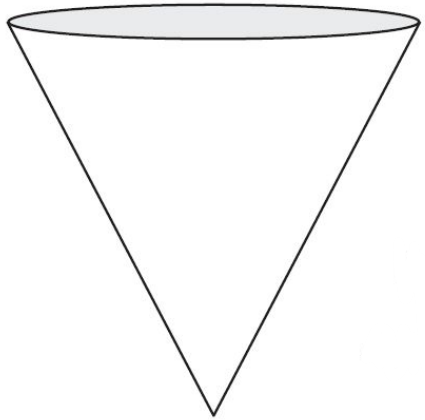
\includegraphics[width=\textwidth]{introductionCone.png}
				\end{center}
			\end{column}
		\end{columns}
	\end{frame}

	\begin{frame}
		\frametitle{Обзор}
		\begin{itemize}
			\item Обзор существующих решений
			\begin{itemize}
				\item Цель и фокус обзора
				\item Критерии сравнения
				\item Таблица с результатами
				\item Выводы
			\end{itemize}
			\item Обзор используемых чужих результатов
			\begin{itemize}
				\item  Всё, написанное и придуманное не вами --- в обзор
			\end{itemize}
			\item Должен соотноситься с темой и с фокусом работы
		\end{itemize}
	\end{frame}

	\begin{frame}
		\frametitle{Описание решения}
		\begin{itemize}
			\item 2-5 разделов
			\begin{itemize}
				\item Желательно, чтобы разделы отвечали решению задачи из списка задач во введении
			\end{itemize}
			\item Аргументированное обоснование принятых решений и отказа от альтернатив
			\item Описание программной реализации
			\begin{itemize}
				\item Выбор инструментария
				\item Архитектура
			\end{itemize}
		\end{itemize}
	\end{frame}

	\begin{frame}
		\frametitle{Описание решения (2)}
		\begin{itemize}
			\item Рисунки и диаграммы
			\begin{itemize}
				\item Лучше использовать UML --- он стандартный
				\item Подписи
				\begin{itemize}
					\item Чужие рисунки --- со ссылкой на источник
				\end{itemize}
				\item Ссылки из текста
				\item Сквозная нумерация
			\end{itemize}
			\item Таблицы
			\begin{itemize}
				\item Чтобы было всё видно даже в напечатанном варианте
			\end{itemize}
		\end{itemize}
	\end{frame}

	\begin{frame}
		\frametitle{Описание решения (3)}
		\begin{itemize}
			\item Сравнение с аналогами
			\item Эксперименты
			\begin{itemize}
				\item Не просто ``Запустил --- работает''
				\item Графики и таблицы
				\item Обязательно подписи к осям, единицы измерения и т.д.
				\item Не забываем матстатистику --- матожидание, дисперсия, доверительные интервалы
				\item Должны соотноситься с целью работы
			\end{itemize}
		\end{itemize}
	\end{frame}

	\begin{frame}
		\frametitle{Описание решения (4)}
		\begin{itemize}
			\item ``Обсуждение''
			\begin{itemize}
				\item Ограничения исследования и валидность (``threats to validity and limitations'')
				\item Возможные альтернативы, ``tradeoffs''
				\item Дальнейшие пути развития
			\end{itemize}
			\item Листингов кода не надо
			\begin{itemize}
				\item Если они важны --- можно, но лучше в приложение
			\end{itemize}
			\item Никакого плагиата! И самоплагиата.
		\end{itemize}
	\end{frame}

	\begin{frame}
		\frametitle{Заключение}
		\begin{itemize}
			\item Перечисление результатов, выносимых на защиту
			\item Должно быть согласовано с постановкой задачи (вплоть до полного её повторения)
			\item Должно быть согласовано с текстом
			\begin{itemize}
				\item Никаких результатов из ниоткуда
			\end{itemize}
			\item Примерно полстраницы
		\end{itemize}
	\end{frame}

	\begin{frame}
		\frametitle{Литература}
		\begin{itemize}
			\item Cсылок примерно как страниц в работе
			\item Обязательно на каждый пункт ссылаться из текста
			\item Лучше ссылаться на научные статьи
			\begin{itemize}
				\item Ещё лучше --- на книги, но по предметной области
				\item Смотрите на индекс Хирша и число цитирований
			\end{itemize}
			\item Реально прочитанные работы
			\begin{itemize}
				\item Всё-таки прочитать бывает полезно
			\end{itemize}
		\end{itemize}
	\end{frame}

	\begin{frame}
		\frametitle{Литература (2)}
		\begin{itemize}
			\item ГОСТ Р 7.0.5-2008
			\begin{itemize}
				\item А.Н. Терехов, Т.А. Брыксин, Ю.В. Литвинов и др., Архитектура среды визуального моделирования QReal. // Системное программирование. Вып. 4. СПб.: Изд-во СПбГУ. 2009, С. 171-196
				\item Порядок --- алфавитный (по авторам), в порядке упоминания в тексте, в хронологическом порядке (если это важно)
				\item Ссылки в тексте --- номер в квадратных скобках: ``блаблабла [1]'' (с пробелом)
			\end{itemize}
			\item В литературу --- только, гм, литературу
			\begin{itemize}
				\item Подстраничные сноски для ссылок на сайты, статьи на хабре и т.д.
				\item Электронные источники в списке литературы допустимы (надо указывать дату обращения)
			\end{itemize}
		\end{itemize}
	\end{frame}

	\begin{frame}
		\frametitle{Презентация, структура}
		\begin{itemize}
			\item Титульный слайд
			\item Введение (примерно 1-2 слайда)
			\item Постановка задачи (1 слайд)
			\item Обзор (примерно 1 слайд)
			\item Предлагаемое решение (примерно 1-2 слайда)
			\item Апробация, эксперименты (примерно 1 слайд)
			\item Результаты, выносимые на защиту (1 слайд) --- обязательно, последним слайдом
		\end{itemize}
	\end{frame}

	\begin{frame}
		\frametitle{FAQ}
		\begin{itemize}
			\item Можно ли писать групповую курсовую?
			\begin{itemize}
				\item Да, но отчёт и презентация у каждого свои
			\end{itemize}
			\item Можно ли брать курсовую не с кафедры?
			\begin{itemize}
				\item Да, кафедра назначит формального научника, фактический руководитель станет \textit{консультантом}
			\end{itemize}
			\item Засчитывают ли выступление на конференции за защиту (предзащиту)?
			\begin{itemize}
				\item Нет
			\end{itemize}
			\item Можно ли менять тему и научника?
			\begin{itemize}
				\item Да, но предупредить куратора
			\end{itemize}
			\item Можно ли перезачесть работу?
			\begin{itemize}
				\item Да, но заранее предупредить куратора
			\end{itemize}
		\end{itemize}
	\end{frame}

	\begin{frame}
		\frametitle{Рассылка про курсовые}
		\begin{Large}
			\begin{center}
				\url{http://bit.ly/se-bachelors-2021}

				Подписаться обязательно!
			\end{center}
		\end{Large}
	\end{frame}

\end{document}